\documentclass[10pt,twocolumn]{article}

%% ── Packages ──────────────────────────────────────────────────────────────
\usepackage{amsmath,amssymb,amsthm}
\usepackage{mathtools}
\usepackage{microtype}


\usepackage{geometry}
\usepackage{hyperref}
\usepackage{natbib}
\usepackage{tikz}
\usetikzlibrary{arrows.meta,positioning,calc}
\usepackage{booktabs}
\usepackage{array}
\usepackage{xcolor}
\usepackage{titlesec}
\usepackage{abstract}
\usepackage{caption}
\usepackage{enumitem}
\usepackage{appendix}

\geometry{
  paperwidth=8.5in, paperheight=11in,
  top=0.85in, bottom=0.9in,
  left=0.65in, right=0.65in,
  columnsep=0.22in
}

\hypersetup{colorlinks=true,linkcolor=black,citecolor=black,urlcolor=black}

%% ── Title formatting ──────────────────────────────────────────────────────
\titleformat{\section}{\normalsize\bfseries}{\thesection.}{0.5em}{}
\titleformat{\subsection}{\small\bfseries}{\thesubsection.}{0.5em}{}
\titleformat{\subsubsection}{\small\itshape}{\thesubsubsection.}{0.4em}{}
\titlespacing{\section}{0pt}{6pt plus 2pt minus 1pt}{3pt plus 1pt}
\titlespacing{\subsection}{0pt}{4pt plus 1pt}{2pt}

%% ── Abstract ──────────────────────────────────────────────────────────────
\renewcommand{\abstractnamefont}{\small\bfseries}
\renewcommand{\abstracttextfont}{\small}
\setlength{\absleftindent}{0pt}
\setlength{\absrightindent}{0pt}

%% ── Theorem environments ──────────────────────────────────────────────────
\theoremstyle{plain}
\newtheorem{theorem}{Theorem}
\newtheorem{proposition}{Proposition}
\newtheorem{lemma}{Lemma}
\newtheorem{corollary}{Corollary}
\theoremstyle{definition}
\newtheorem{definition}{Definition}
\theoremstyle{remark}
\newtheorem{remark}{Remark}

%% ── Shorthands ────────────────────────────────────────────────────────────
\newcommand{\simA}{\sim_{\!A}}
\newcommand{\simO}{\sim_{\!O}}
\newcommand{\simC}{\sim_{\!C}}
\newcommand{\simI}{\sim_{\!I}}
\newcommand{\RHP}{\mathcal{R}_{H}^{\Pi}}
\newcommand{\DA}{D_{A}(\varphi)}
\newcommand{\calX}{\mathcal{X}}
\newcommand{\calM}{\mathcal{M}}
\newcommand{\Xmod}[1]{\calX/{\sim_{#1}}}

%% ── Caption setup ─────────────────────────────────────────────────────────
\captionsetup{font=small,labelfont=bf,skip=4pt}

%% ── Spacing ───────────────────────────────────────────────────────────────
\setlength{\parskip}{2pt}
\setlength{\abovedisplayskip}{4pt}
\setlength{\belowdisplayskip}{4pt}

% ═══════════════════════════════════════════════════════════════════════════
\title{\textbf{Against Latent Fundamentalism}\\[2pt]
  {\normalsize\itshape Admissibility Distortion and the Missing Criterion
  in Representation Learning for Planning}}

\author{Flyxion\\
  {\small Independent Researcher}\\
  {\small \texttt{github.com/standardgalactic}}}

\date{}

% ═══════════════════════════════════════════════════════════════════════════
\begin{document}
\maketitle
\thispagestyle{plain}

% ── Abstract ──────────────────────────────────────────────────────────────
\begin{abstract}
\noindent
Representation learning for planning lacks a principled criterion for whether a
learned projection preserves the distinctions planning requires. We identify that
criterion: \emph{admissibility distortion} $\DA$, which equals zero if and only
if the projection is admissibility-preserving. The admissibility equivalence
relation $\simA$---the coarsest relation compatible with adequate planning---is
derived from planning requirements alone, not from reward structure, observation
statistics, or architectural choices. The central result, the
\emph{Observational--Interventional Separation Theorem}, establishes that
$\simO \not\Rightarrow \simI$ in general: this is a structural mismatch between
equivalence-generating operations, not an empirical contingency. Three corollaries
follow: predictive projections satisfy $D_{A}(\varphi_{P})\not\equiv 0$ in
general; compressive projections satisfy $D_{A}(\varphi_{C})\not\equiv 0$; and
by the data-processing inequality, any downstream guardrail classifier is bounded
above by $I(A;\varphi(X))$, with a Fano-derived Bayes-risk floor that is
independent of classifier complexity. A collapse--separation decomposition
($\DA = P(C_{\varphi}{=}1)\,\mathbb{E}[\Delta_{A}\mid C_{\varphi}{=}1]$)
distinguishes broad-compressive from catastrophic-blind-spot failure modes.
Trajectory-sampling lower bounds enable witnessed violation detection without full
dynamics access: any collapsed pair whose reachability sets disagree under a
sampled policy proves $\DA>0$. Admissibility distortion is
a foundational target criterion, not yet an engineering metric; the contribution
is naming the missing quantity and deriving its properties.
\end{abstract}

\smallskip
\noindent\textbf{Keywords:} representation learning, state abstraction, reachability,
admissibility, planning, safety, world models.

% ═══════════════════════════════════════════════════════════════════════════
\section{Introduction}
\label{sec:intro}

Planning requires choosing among actions by evaluating their consequences.
Any representation intended to support planning must therefore preserve, at
minimum, the distinctions that determine which futures are accessible. When a
representation fails to preserve such distinctions, planning errors follow that
cannot be corrected by improving the optimiser, refining the cost function, or
adding safety machinery---the failure is logically prior to all of those
operations.

Current representation-learning objectives---predictive accuracy, information
maximisation, compression progress, contrastive separation---optimise for
properties of the observation distribution. None directly optimises for
preservation of reachability structure. The question of whether a given latent
space is adequate for planning is therefore not addressed by any current training
objective; it is at best hoped that predictive or compressive objectives will be
admissible incidentally.

We show that the missing criterion is \emph{admissibility distortion} $\DA$. The
argument has a fixed logical architecture: planning induces $\simA$; $\simA$
induces $\DA$; and existing objectives are evaluated by how well they approximate
$\mathcal{X}/\simA$. The paper's contributions are (i) the derivation of $\simA$
and $\DA$ from planning requirements without reference to reward or observations;
(ii) the Observational--Interventional Separation Theorem establishing that the gap
is structural, not empirical; (iii) three corollaries for prediction, compression,
and safety; (iv) a decomposition theorem and trajectory-sampling lower bound for
diagnostic use; and (v) a formal asymmetry result showing that positive lower-bound
estimates witness genuine violations while zero estimates provide no certificate.

\textit{Relation to prior work.} The earliest precise statement of the world-model
concept appears in \citet{craik1943nature}, who argued that an organism carrying
``a small-scale model of external reality and its own possible actions within its
head'' can ``try out various alternatives'' and ``react to future situations before
they arise.'' Craik's formulation already identifies what we formalise as
reachability structure: the model must represent the agent's \emph{possible
actions}, not merely passive observations of the world. The state-abstraction programme
\citep{li2006towards,ravindran2004algebraic} asks which collapses are safe for
policy quality; admissibility extends this beyond value-function equivalence to
reachability-set equivalence. Bisimulation metrics \citep{ferns2004metrics,
castro2010bisimulation,kemertas2021towards,zhang2021learning} provide continuous
relaxations; Proposition~\ref{prop:bisim_bound} shows these are lower bounds on
$\DA$. Predictive state representations \citep{littman2002predictive} and general
value functions \citep{sutton2011horde} encode prediction structure; the
separation theorem shows this is insufficient. Pearl's do-calculus
\citep{pearl2009causality} formalises observation vs.\ intervention; our theorem
is the planning-theoretic analogue. The information bottleneck
\citep{tishby1999information} minimises $I(X;Z)$ subject to $I(Z;Y)$; replacing
$Y$ with the admissibility signal yields an admissibility-constrained bottleneck.
Gibson's affordance theory \citep{gibson1979ecological} shifts representation
from object identity to action possibility, as does $\simA$. Model predictive
control \citep{mayne2000model,garcia1989model} and reachability analysis
\citep{tomlin2003computational} assume state representations are already adequate;
$\DA$ formalises when that assumption fails. Controllability Gramians and
reachability metrics in linear control theory \citep{kalman1960general} provide
task-specific admissibility criteria under Gaussian dynamics; $\simA$ generalises
these to arbitrary policy classes without linearity assumptions.
Information-state representations in POMDPs \citep{kaelbling1998planning} preserve
sufficient statistics for optimal planning under partial observability; extending
$\simA$ to belief-space reachability connects these frameworks and is a natural
direction for future work.

% ═══════════════════════════════════════════════════════════════════════════
\section{Planning Induces Admissibility}
\label{sec:planning}

\subsection{Setup and Reachability}

Let $\calX$ be a state space, $H\in\mathbb{N}$ a planning horizon, and $\Pi$
a policy class. Write $x \overset{\pi,h}{\rightsquigarrow} y$ when state $y$
is reachable from $x$ in $h$ steps under policy $\pi$. This formalises what
\citet{craik1943nature} called the capacity to ``try out various alternatives''
before acting: the reachability set is exactly the set of alternatives available
to the agent.

\begin{definition}[Reachability Set]
\label{def:reach}
$\RHP(x) = \{y\in\calX : \exists\,\pi\in\Pi,\; x\overset{\pi,H}{\rightsquigarrow}y\}$.
\end{definition}

\begin{proposition}[Planning Sufficiency Requirement]
\label{prop:planning}
If $\RHP(x_1)\neq\RHP(x_2)$, there exists a planning problem for which the
optimal policy from $x_1$ differs from the optimal policy from $x_2$. Hence any
representation adequate for planning must distinguish states with distinct
reachability sets.
\end{proposition}

\noindent(Proof in Appendix~\ref{app:proofs}.)

\subsection{Admissibility Equivalence and Distortion}

\begin{definition}[Admissibility Equivalence]
\label{def:admissibility}
$x_1 \simA x_2 \iff \RHP(x_1) = \RHP(x_2)$.
A projection $\varphi:\calX\to\calM$ is \emph{admissible} if
$\varphi(x_1)=\varphi(x_2)\Rightarrow x_1\simA x_2$.
\end{definition}

The relation $\simA$ is derived, not assumed: it is the coarsest equivalence
relation on $\calX$ consistent with Proposition~\ref{prop:planning}. This gives
it the character of a sufficient statistic \citep{fisher1922mathematical}: it is
the minimally discriminative representation safe for all accessibility-structured
planning tasks.

\begin{remark}[Capability-relativity]
\label{rem:relativity}
$\simA$ is properly written $\sim_A^{(\Pi,H)}$: it depends on the agent's
capability class $\Pi$ and planning horizon $H$. This is not a deficiency.
Every useful equivalence relation in planning is similarly indexed: bisimulation
depends on transition structure, observability depends on sensors, controllability
depends on actuators. If an agent acquires new capabilities, $\Pi$ expands and
$\simA$ may split previously equivalent pairs, requiring finer representation.
Admissibility is intentionally relative to a capability class: a representation
adequate for one class need not remain adequate for a strictly larger one.
\end{remark}

\begin{definition}[Admissibility Distortion]
\label{def:distortion}
\begin{equation}
  \DA \;=\; \mathbb{E}_{x_1,x_2}\!\left[
    \mathbf{1}_{\varphi(x_1)=\varphi(x_2)}
    \cdot d\!\left(\RHP(x_1),\RHP(x_2)\right)
  \right],
\end{equation}
where $d(\cdot,\cdot)$ is any metric on subsets of $\calX$ (e.g.\ Hausdorff
distance) and the expectation is over pairs drawn from the agent's state
distribution. $\DA=0$ iff $\varphi$ is admissible.
\end{definition}

\begin{remark}[Metric invariance of the binary question]
\label{rem:metricinv}
The question $\DA=0$ versus $\DA>0$ is invariant under any choice of $d$
satisfying $d(S,T)=0\iff S=T$. The metric affects only the severity weighting
assigned to violations, not whether they exist. All theorem-level results
(separation, monotonicity, irrecoverable collapse) concern the binary question
and are therefore metric-independent.
\end{remark}

\begin{theorem}[Zero-Distortion Characterisation]
\label{thm:char}
$\DA = 0 \iff P\!\left(C_\varphi(x_1,x_2)=1,\; x_1\not\simA x_2\right) = 0.$
That is, admissibility distortion vanishes iff collapsed pairs are
admissibility-equivalent almost surely.
\end{theorem}

\noindent(Proof in Appendix~\ref{app:proofs}.)

\begin{remark}[Epistemic status]
$\DA$ is mathematically well-defined but not computable in full generality
without access to the dynamics in the form needed to enumerate $\RHP(x)$.
The paper treats $\DA$ as a \emph{target criterion}---the quantity representation
learning should minimise---rather than a deployed metric. It plays the role that
Kolmogorov complexity plays in compression theory: foundationally clarifying and
practically directive without being directly computable in general.
\end{remark}

\subsection{Decomposition}

Define the collapse indicator $C_\varphi(x_1,x_2)=\mathbf{1}_{\varphi(x_1)=\varphi(x_2)}$
and reachability separation $\Delta_A(x_1,x_2)=d(\RHP(x_1),\RHP(x_2))$.

\begin{proposition}[Collapse--Separation Decomposition]
\label{prop:decomp}
$\DA = P(C_\varphi=1)\cdot\mathbb{E}[\Delta_A\mid C_\varphi=1].$
\end{proposition}

The decomposition distinguishes two failure modes: \emph{broad-compressive} failure
(high $P(C_\varphi=1)$, moderate $\mathbb{E}[\Delta_A\mid C_\varphi=1]$) and
\emph{catastrophic blind-spot} failure (low $P(C_\varphi=1)$, but the few merged
pairs have $\Delta_A\gg 0$). Two representations with equal $\DA$ may call for
entirely different interventions.

\subsection{Universality and Monotonicity}

\begin{theorem}[Universality of $\simA$]
\label{thm:universality}
Let $\mathfrak{T}_A$ be the class of \emph{accessibility tasks}: cost functions
depending only on which futures are reachable, not on transition probabilities or
reward magnitudes along trajectories. Then
$\simA = \bigcap_{\mathcal{T}\in\mathfrak{T}_A}\sim_{\mathcal{T}}$,
where $x_1\sim_\mathcal{T} x_2$ iff the optimal policies from $x_1$ and $x_2$
coincide under $\mathcal{T}$. Consequently $\simA$ is the largest equivalence
relation safe for all tasks in $\mathfrak{T}_A$.
\end{theorem}

\begin{remark}[Scope of universality]
Tasks whose costs depend on transition \emph{probabilities} or reward magnitudes
(rather than mere reachability) may distinguish states that $\simA$ identifies.
For such tasks, admissibility must be extended to an \emph{admissibility profile}
recording reachable states together with their access-cost distributions; this
extension is deferred to future work. The present results establish $\simA$ as a
necessary condition for all tasks in $\mathfrak{T}_A$, which includes all
goal-conditioned and viability objectives.
\end{remark}

\begin{theorem}[Monotonicity]
\label{thm:monotone}
If ${\sim_{\varphi_1}}\subseteq{\sim_{\varphi_2}}$ (so $\varphi_2$ collapses at
least every pair $\varphi_1$ collapses), then $D_A(\varphi_1)\leq D_A(\varphi_2)$.
\end{theorem}

Let $\mathcal{N}={\sim_{\varphi_2}}\setminus{\sim_{\varphi_1}}$ denote newly
collapsed pairs.

\begin{corollary}[Accounting Identity]
\label{cor:accounting}
$D_A(\varphi_2) - D_A(\varphi_1) = \mathbb{E}[\mathbf{1}_{\mathcal{N}}(x_1,x_2)
\cdot \Delta_A(x_1,x_2)].$
\end{corollary}

The increase in distortion from any compression step is exactly the expected
reachability separation of the newly merged pairs---not a bound, but an identity.
This makes the admissibility cost of each compression decision explicit and in
principle auditable.

\begin{corollary}[Strict Monotonicity]
\label{cor:strict}
If there exists a pair $(x_1,x_2)\in\mathcal{N}$ with $\Delta_A(x_1,x_2)>0$
on a set of positive measure, then $D_A(\varphi_2) > D_A(\varphi_1)$.
\end{corollary}

\noindent(Immediate from Corollary~\ref{cor:accounting}: the expectation is
strictly positive when a positive-measure set of newly merged pairs have nonzero
separation.) This identifies exactly when compression increases distortion: it
does so whenever any newly merged pair consists of states with genuinely different
reachable futures.

\begin{proposition}[Lipschitz Stability]
\label{prop:lipschitz}
Suppose reachability sets are Lipschitz in the state metric: $d_H(\RHP(x_1),
\RHP(x_2))\leq L\,d_\calX(x_1,x_2)$ for some $L>0$ and state metric $d_\calX$.
Then
\[
  \DA \;\leq\; L\;\mathbb{E}\!\left[
    \mathbf{1}_{C_\varphi=1}\cdot d_\calX(x_1,x_2)
  \right].
\]
\end{proposition}

\noindent(Proof: substitute the Lipschitz bound into Definition~\ref{def:distortion}.)
This connects admissibility distortion to geometric clustering: any encoder that
collapses only nearby states (small $d_\calX$ between merged pairs) has controlled
distortion under the Lipschitz assumption. It also provides a surrogate objective:
penalise the expected state-space distance between collapsed pairs.

The implications are sharper than the familiar observation that lossy compression
discards information. There exists a partial order on representations under which
improving compression efficiency \emph{monotonically} increases admissibility risk.
Compression objectives unconstrained by admissibility exert structural pressure
toward admissibility-violating identifications, strongest on rare high-consequence
states---precisely the distinctions that appear as noise to the compressor but
determine reachability at the boundaries that matter most.

% ═══════════════════════════════════════════════════════════════════════════
\section{Observational--Interventional Separation}
\label{sec:oi}

\begin{definition}[Observational Equivalence]
$x_1\simO x_2$ if $P(O_{t+1:t+k}\mid X_t=x_1)=P(O_{t+1:t+k}\mid X_t=x_2)$
for all $k\geq 1$ under a fixed observational policy.
\end{definition}

\begin{definition}[Interventional Equivalence]
$x_1\simI x_2$ if $\{y:x_1\overset{\pi,h}{\rightsquigarrow}y\}=\{y:x_2\overset{\pi,h}{\rightsquigarrow}y\}$
for all $\pi\in\Pi$, $h\leq H$.
\end{definition}

\begin{proposition}
\label{prop:id}
$\simI = \simA$.
\end{proposition}

\begin{theorem}[Observational--Interventional Separation]
\label{thm:oi}
In general, $\simO \not\Rightarrow \simI$: there exist states
$x_1,x_2\in\calX$ that are observationally equivalent but interventionally
inequivalent.
\end{theorem}

\noindent\textit{Canonical example.} Let $x_1$ be a structurally intact
load-bearing element and $x_2$ the same element with an internal crack invisible
to surface sensors. Under passive observation, $P(O\mid x_1)=P(O\mid x_2)$, so
$x_1\simO x_2$. Under a policy applying stress beyond the crack threshold,
$x_2$ admits failure states unreachable from $x_1$: $\RHP(x_1)\neq\RHP(x_2)$,
so $x_1\not\simI x_2$.

\begin{remark}[Structural mismatch]
\label{rem:mismatch}
The theorem identifies a \emph{structural mismatch between equivalence-generating
operations}: $\simO$ compares probability measures over passive observation
sequences; $\simI$ compares subsets of $\calX$ under arbitrary interventions.
These are different mathematical objects. The gap cannot be closed by improving
the predictive model, collecting more data, or shifting prediction from pixel
space to latent space, because none of those operations changes the type of the
equivalence relation being computed. The theorem targets \emph{passive}
representation learning; agents that act and observe outcomes generate
interventional data and can in principle close the gap, but this requires active
exploration, not self-supervised prediction.
\end{remark}

The theorem is the planning-theoretic analogue of Pearl's do-calculus
\citep{pearl2009causality}: $P(Y\mid X=x)\neq P(Y\mid\mathrm{do}(X=x))$ in
general; correspondingly, $\simO\neq\simI$ in general. It also formalises the
identification--reachability gap in control theory \citep{ljung1999system}: system
identification yields observational accuracy but not necessarily control adequacy.
Both gaps are instances of a deeper inversion problem: the equivalence relation
that passive observation generates is the wrong type for the question being asked.
Standard frequentist methodology faces an exactly analogous inversion---it
computes $P(\text{data}\mid\text{hypothesis})$ when the scientifically relevant
quantity is $P(\text{hypothesis}\mid\text{data})$, and no accumulation of
observational data resolves the type mismatch \citep{jaynes2003probability}.
The $\simO$/$\simA$ separation is the geometric form of this inversion: learners
receive observations and compute observational partitions, but planning requires
reachability partitions, and these are different mathematical objects.

A characterisation theorem (Appendix~\ref{app:proofs}) identifies precisely when
coincidence holds: $\simO\subseteq\simA$ iff every intervention-relevant variable
is observationally identifiable. This is an \emph{additional} structural property
of the system, not a consequence of predictive training. Verifying it is an
independent problem that no current objective addresses.

% ═══════════════════════════════════════════════════════════════════════════
\section{Three Corollaries}
\label{sec:corollaries}

\subsection{Predictive Gap}

\begin{corollary}[Predictive Admissibility Gap]
\label{cor:pred}
If $\varphi_P$ collapses $x_1\simO x_2$, then $D_A(\varphi_P)\not\equiv 0$
in general.
\end{corollary}

By Theorem~\ref{thm:oi}, there exist $x_1\simO x_2$ with $\RHP(x_1)\neq\RHP(x_2)$.
Any predictive projection identifying them contributes positively to $D_A(\varphi_P)$.
This applies equally to contrastive predictive coding \citep{oord2018representation},
successor representations \citep{dayan1993improving}, and general value functions
\citep{sutton2011horde}: all encode future observation structure; all are subject
to the predictive gap. Moving prediction from pixel space to latent space changes
the domain of prediction without changing the type of the equivalence relation.

\subsection{Compression Gap}

\begin{corollary}[Compression Admissibility Gap]
\label{cor:comp}
$D_A(\varphi_C)\not\equiv 0$ in general for any projection $\varphi_C$
minimising description length.
\end{corollary}

By Theorem~\ref{thm:monotone} and Corollary~\ref{cor:accounting}, each compression
step incurs additional distortion equal to the expected separation of newly merged
pairs. The information bottleneck \citep{tishby1999information} specialises this:
a representation that maximally compresses toward an observed reward signal may
discard admissibility-relevant structure if that structure is uncorrelated with
the reward in the training distribution.

\subsection{Guardrail Incompleteness and Bayes-Risk Floor}

\begin{corollary}[Safety--Admissibility Gap]
\label{cor:safety}
If $\DA > 0$ because $\varphi(x_s)=\varphi(x_d)$ for safe $x_s$ and dangerous
$x_d$, then no guardrail classifier operating on $\calM$ alone (without temporal
context, action history, or post-hoc outcome information) can distinguish them.
\end{corollary}

\noindent\textit{Constructive proof.} Any $G:\calM\to\{0,1\}$ satisfies
$G(\varphi(x_s))=G(\varphi(x_d))$ since both equal $G(z)$ for $z=\varphi(x_s)=\varphi(x_d)$.
One state is necessarily misclassified. The failure is a consequence of the
projection, not of classifier architecture or capacity. Monitors with access to
action sequences or outcome histories may use information beyond $\varphi(x)$
and are not subject to this bound; the corollary applies to any classifier whose
inputs are restricted to the latent representation at a single time step.

\begin{theorem}[Irrecoverable Quotient Collapse]
\label{thm:guardrail}
Let $A\in\{0,1\}$ indicate admissibility status. For every downstream
transformation $G:\calM\to\{0,1\}$,
\begin{equation}
  I\!\left(A;\,G(\varphi(X))\right) \;\leq\; I\!\left(A;\,\varphi(X)\right).
\end{equation}
If $I(A;\varphi(X))=0$, then $I(A;G(\varphi(X)))=0$ for all $G$.
\end{theorem}

\noindent(Proof in Appendix~\ref{app:proofs}.) This provides a principled
diagnostic: persistent safety failure with error near $0.5$ is attributable to
the representation rather than the classifier architecture.

\begin{corollary}[Bayes-Risk Floor]
\label{cor:bayes}
Let $Z=\varphi(X)$. The Bayes error of any binary classifier distinguishing
$A\in\{0,1\}$ from $\varphi(X)$ satisfies
\begin{equation}
  \varepsilon^* \;=\; \mathbb{E}_{Z}\!\left[\min\!\left\{
    P(A=0\mid Z),\; P(A=1\mid Z)
  \right\}\right].
\end{equation}
When $I(A;\varphi(X))$ is low, conditional uncertainty $H(A\mid Z)$ is high,
and $\varepsilon^*$ approaches $\min(p,1-p)$ where $p=P(A=1)$. If $p\approx 0.5$,
$\varepsilon^*\to 0.5$: any safety classifier on such a projection performs
near-randomly regardless of its complexity.
\end{corollary}

% ═══════════════════════════════════════════════════════════════════════════
\section{Representation Learning as Quotient Selection}
\label{sec:quotient}

\begin{proposition}[Quotient Framing]
\label{prop:quotient}
Every representation-learning method induces an equivalence relation
${\sim_\varphi}$ on $\calX$ and thereby proposes a quotient $\Xmod{\varphi}$.
The admissibility question is, in every case, whether ${\sim_\varphi}\subseteq\simA$.
\end{proposition}

Anti-trivial-collapse mechanisms (EMA encoders, VICReg, contrastive terms)
constrain the global distribution of equivalence classes without constraining
which states are identified. They prevent $|\Xmod{\varphi}|=1$ but do not enforce
${\sim_\varphi}\subseteq\simA$.

The disputes among JEPA, latent diffusion, transformer world models, bisimulation
learning, and compression-based intelligence are, at this level of description,
disputes about quotient selection. The renormalisation-group perspective
\citep{wilson1975renormalization} asks which distinctions survive coarse-graining;
admissibility inverts this: which distinctions \emph{must not} be coarse-grained?

% ═══════════════════════════════════════════════════════════════════════════
\section{Admissibility as Prior Condition}
\label{sec:prior}

The admissibility framework is not a competing objective: it is a prior condition
derived from what planning requires, not assumed as a desideratum. Every planning
goal---prediction, compression, control, reward, safety---presupposes that distinct
futures can be distinguished and that some are accessible while others are not.
Admissibility formalises that presupposition.

The claim is a necessary-condition claim, not a sufficiency claim. A system with
$\DA\approx 0$ may still fail at understanding, consciousness, or adaptability for
reasons this framework does not address. The framework claims only that $\DA>0$
is sufficient for planning failure, and that $\DA=0$ is necessary for adequate
planning. This necessary condition is universal: it applies with equal force to
biological nervous systems, social institutions, and artificial systems. A human
planner who systematically confuses states with different reachable futures incurs
planning failures by the same mechanism as a neural network with high $\DA$.

Model predictive control \citep{mayne2000model,garcia1989model} presupposes that
state variables are already correctly chosen---that the representation is a
sufficient statistic for future evolution. The novel claim of JEPA-based world
models is that self-supervised latent representations constitute such sufficient
statistics. Corollary~\ref{cor:pred} establishes that this claim is unproven and
that the criterion by which it could be evaluated is precisely $\DA$.

% ═══════════════════════════════════════════════════════════════════════════
\section{Toward Estimation}
\label{sec:estimation}

\subsection{Foundational status}

$\DA$ is not yet an engineering metric. It is a target criterion. The contribution
of this paper is not an estimator; it is the identification of the quantity whose
estimation future work must address. The research agenda is: develop estimators
that are eventually tight in expectation, and certificates that are eventually
sound.

\subsection{Bisimulation lower bound}

\begin{proposition}
\label{prop:bisim_bound}
Let $D_{\mathrm{bisim}}(\varphi)$ be the bisimulation distortion of $\varphi$
under reward functions depending only on reachability. Then
$D_{\mathrm{bisim}}(\varphi)\leq C\cdot\DA$ for a constant $C$ depending on
reward scale and discount factor. In particular, $\DA=0$ implies
$D_{\mathrm{bisim}}(\varphi)=0$.
\end{proposition}

Bisimulation metrics \citep{ferns2004metrics,kemertas2021towards} thus provide
computable lower bounds on $\DA$.

\subsection{Trajectory-sampling lower bound}

Fix $\Pi_k=\{\pi_1,\ldots,\pi_k\}\subseteq\Pi$. Define the
\emph{witnessed-disagreement indicator} for a collapsed pair as
\[
  W_k(x_1,x_2) = \mathbf{1}\!\left[\exists\,\pi_i\in\Pi_k :\;
    \hat{\mathcal{R}}^{\pi_i,H}(x_1)\neq\hat{\mathcal{R}}^{\pi_i,H}(x_2)
  \right],
\]
where $\hat{\mathcal{R}}^{\pi_i,H}(x)=\{y:x\overset{\pi_i,H}{\rightsquigarrow}y\}$.
Define the \emph{witnessed distortion}
\[
  \hat{D}_A(\varphi;\Pi_k) = \mathbb{E}\!\left[
    \mathbf{1}_{C_\varphi=1}\cdot W_k(x_1,x_2)
  \right].
\]

\begin{proposition}[Trajectory Lower Bound]
\label{prop:lower_bound}
$\hat{D}_A(\varphi;\Pi_k)\leq \mathbf{1}_{D_A(\varphi)>0}$ in the sense that
$\hat{D}_A(\varphi;\Pi_k)>0$ implies $\DA>0$: any witnessed disagreement between
collapsed states proves admissibility distortion exists. This bound does not
require any metric monotonicity assumption.
\end{proposition}

\begin{proposition}[Asymmetry of Evidence]
\label{prop:asymmetry}
(i) If $\hat{D}_A(\varphi;\Pi_k)>0$, then $\DA>0$: any witnessed reachability
disagreement between collapsed states \emph{proves} distortion exists. (ii) If
$\hat{D}_A(\varphi;\Pi_k)=0$, this does not imply $\DA=0$: a zero result proves
only that the sampled policies found no witness.
\end{proposition}

The asymmetry is that of model checking and adversarial testing: finding a
counterexample is definitive; failing to find one is not a proof of correctness.
Trajectory-sampling audits are one-sided diagnostic tools whose value increases
with the adversarial diversity of $\Pi_k$.

\subsection{Structural vs.\ operational distortion}

Operational distortion $D_A^\pi(\varphi)$ is the expectation over states visited
by the current policy; structural distortion $D_A^{\mathrm{struct}}(\varphi)=
\sup_{x_1,x_2}\mathbf{1}_{C_\varphi=1}\cdot\Delta_A(x_1,x_2)$ measures the
worst case over $\calX$. These can diverge dramatically: $D_A^\pi\approx 0$
under a conservative policy while $D_A^{\mathrm{struct}}\gg 0$ in rarely-visited
regions. Safety-critical failures characteristically occur in low-frequency,
high-consequence regions that operational distortion underweights.

\subsection{Task-weighted distortion}

A task-weighted refinement
$D_A^w(\varphi)=\mathbb{E}[w(x_1,x_2)\cdot\mathbf{1}_{C_\varphi=1}\cdot\Delta_A(x_1,x_2)]$
interpolates between operational and structural distortion when $w$ assigns high
weight to safety-critical regions regardless of visit frequency. The conflict
between compression and admissibility is sharpest when the probability measure
over states and the importance weights over states are systematically opposed,
as they are in safety-critical domains.

\subsection{Admissibility depth}

\begin{definition}[Admissibility Depth]
$d_A(x_1,x_2)=\min\{H:\RHP[H](x_1)\neq\RHP[H](x_2)\}$, with $d_A=\infty$
if $x_1\simA x_2$ for all $H$.
\end{definition}

The horizon hierarchy $\sim_A^{(\Pi,1)}\supseteq\sim_A^{(\Pi,10)}\supseteq\cdots$
implies that representations adequate for one-step prediction may be
catastrophically inadmissible for strategic planning.

% ═══════════════════════════════════════════════════════════════════════════
\section{Discussion}
\label{sec:discussion}

\textit{Scope conditions.} The framework presupposes a fixed $(\calX,\Pi,H)$.
When a system alters its own element types---new variables become relevant, old
ones disappear---$\simA$ must be re-derived on the enlarged or altered space.
This challenge is shared by every formal framework that requires a domain before
analysis can begin. The admissibility framework is better positioned than
distributional approaches: since $\simA$ is derived from planning requirements
rather than training statistics, it does not presuppose a representative training
distribution. Dynamic state-space evolution is an open problem for the field, not
a special failure of admissibility-based approaches.

\textit{Relation to impossibility arguments.} Arguments that intelligence is
impossible to formalise because complex systems alter their own coordinate systems
are addressed by the above scope observation. The admissibility relation is defined
over reachability geometry, not distributional regularity; non-ergodicity does not
preclude well-defined reachability cones. The relevant objection is not
``irregularity implies impossible'' but ``changing coordinate systems complicate
re-derivation of $\simA$''---a genuine difficulty that converts a putative
refutation into an open research problem.

\textit{Self-modifying agents.} An agent undergoing internal transformation
(updated representations, goals, or memories) remains a coherent agent insofar as
the transformation preserves reachability-relevant distinctions. Narrative identity
frameworks and symbolic stabilisers can be interpreted as mechanisms for
maintaining low $\DA$ across developmental transitions, rather than alternatives
to reachability-based accounts. Graziano's Attention Schema Theory
\citep{graziano2013consciousness} provides a complementary angle: the model-of-the-world
processor that tracks the agent's own attentional states is, in admissibility
terms, tracking which of the agent's own reachable futures remain accessible
given its current attention allocation. A low-distortion self-schema is a
necessary condition for the attention schema to guide action reliably.

\textit{Relation to the Conscious Turing Machine.} \citet{blum2022conscious}
define a formal seven-tuple model of consciousness in which a global broadcast
mechanism (the Down Tree) simultaneously delivers a winning chunk to all
long-term-memory processors. The chunk is selected by a probabilistic Up Tree
tournament weighted by processor confidence. In admissibility terms, the
broadcast mechanism is planning-adequate only if the chunk-selection process
preserves $\simA$: two starting states whose reachable futures differ must not
produce the same winning chunk. If the chunk representation (the \emph{Brainish}
gist) is inadmissible---if it collapses states with distinct reachability
cones---then Corollary~\ref{cor:safety} applies: no downstream processor can
recover the lost distinction, and the system's behaviour from those states will
converge regardless of their different reachable futures. The CTM's subjective
experience, grounded in the co-evolution of Brainish and a world model
\citep{blum2022conscious}, is therefore admissibility-dependent: a genuine
first-person perspective, in \citeauthor{varela1999first}'s sense of ``lived
experience associated with cognitive and mental events''
\citep{varela1999first}, requires that the internal language preserve the
distinctions that determine what the agent can do next.

\textit{Relation to Gupta \& Pruthi.} \citet{gupta2025world} argue that world
models fail to capture understanding because state-tracking is insufficient for
grasping the organising principles that make states significant. The admissibility
framework formalises this diagnosis: the quantity world models fail to preserve
is $\DA$, the departure of the learned quotient from $\Xmod{A}$. Poincar\'e's
distinction between verifying a proof step-by-step and understanding why those
steps were chosen \citep{poincare1914} maps onto Theorem~\ref{thm:oi}: verification
is observational (local transition checking); understanding is interventional
(grasping the reachability geometry of proof space).

\textit{Biological instantiation: photosynthesis--growth decoupling in oaks.}
A recent empirical study of North American temperate deciduous oaks provides
what may be the clearest natural-system instantiation of the
Observational--Interventional Separation Theorem outside of engineering
\citep{rao2026decoupled}. The authors demonstrate that gross primary
productivity (GPP)---the observational quantity accessible to passive remote
sensing, eddy covariance, and satellite fluorescence retrieval---and
aboveground woody biomass growth---the quantity determining long-term carbon
sequestration and thus the accessible futures of the ecosystem---are
systematically decoupled across diel, seasonal, and interannual timescales.
Across 137 tree-ring sites, 26--36\% of annual GPP occurred after July,
yet late-season climate contributed negligibly to annual ring-width variance.
At four high-resolution monitoring sites, growth ceased 2--4 months before
photosynthesis. At the daily scale, growth occurred primarily between midnight
and 07:00 when VPD and temperature were minimal, while GPP peaked near solar
noon under conditions of high atmospheric dryness.

The mechanistic explanation instantiates the coincidence-conditions theorem
(Appendix~\ref{app:proofs}): observational equivalence implies interventional
equivalence only when every intervention-relevant variable is observationally
identifiable. Turgor pressure in cambial cells---the proximate driver of
radial growth---is governed primarily by VPD and stem water status. GPP is
governed primarily by light availability, stomatal conductance, and enzyme
kinetics. These are different state variables subject to different biophysical
constraints, and passive observation of carbon flux cannot identify which
turgor state the cambium is in. Two oaks with identical GPP traces may
therefore have radically different growth futures depending on their hydraulic
status---exactly the structure of $x^h \simO x^f$ but $x^h \not\simA x^f$
in Theorem~\ref{thm:oi}. Earth system models that conflate the photosynthetic
season with the growing season are, in admissibility terms, using an
inadmissible encoder: the learned quotient collapses states whose reachable
futures---measured in woody carbon accumulated over decades---are substantially
different.

The reported Spearman correlation $r = 0.86$ between interannual VPD
variability and the degree of photosynthesis--growth decoupling
\citep{rao2026decoupled} is an empirical measure of how admissibility
distortion in the GPP representation scales with the activation of the
latent constraint variable. As atmospheric aridity becomes more variable,
the gap between observational and interventional equivalence widens---which
is precisely what the framework predicts when a latent variable (turgor
constraint) becomes more dynamically relevant. The monotonicity theorem
(Theorem~\ref{thm:monotone}) further applies to the temporal aggregation
practiced by ESMs: each step of coarsening from hourly to daily to seasonal
to annual GPP is a compression step in the quotient lattice, and
Corollary~\ref{cor:accounting} identifies the admissibility cost as the
expected reachability separation of the pairs each compression step newly
merges. \citeauthor{rao2026decoupled} measure this cost directly: at annual
resolution, post-July GPP carries near-zero information about annual
ring-width, meaning the compression to annual totals has destroyed the
phenological distinction between the growth window and the photosynthetic
season entirely.

% ═══════════════════════════════════════════════════════════════════════════
\section{Conclusion}
\label{sec:conclusion}

We have identified $\DA$ as the missing criterion in representation learning for
planning, derived its properties from planning requirements alone, and established
that predictive and compressive objectives fail to satisfy it in general. The
Observational--Interventional Separation Theorem shows the failure is structural;
the data-processing inequality and Fano bound convert it into operational safety
limits; the decomposition and trajectory-sampling results provide diagnostic
tools. $\DA$ joins the tradition of quantities---entropy, Kolmogorov complexity,
mutual information, Wasserstein distance---that became organising centres for
research programmes by naming something previously unmeasured. The contribution
is not a new architecture or training procedure; it is the identification of a
missing criterion and the derivation of its properties from first principles.

\bigskip
\noindent\textbf{Acknowledgements.} The author has no institutional affiliation
and no conflicts of interest.

% ═══════════════════════════════════════════════════════════════════════════
% APPENDICES
% ═══════════════════════════════════════════════════════════════════════════

\appendix
\renewcommand{\thesection}{\Alph{section}}
\titleformat{\section}{\normalsize\bfseries}{Appendix~\thesection.}{0.5em}{}

\section{Proofs of All Results}
\label{app:proofs}

We collect complete proofs of all propositions, theorems, and corollaries in the
order of their appearance in the main text. Notation follows the main text
throughout.

\subsection*{Proposition~\ref{prop:planning} (Planning Sufficiency Requirement)}

\begin{proof}
Suppose $\RHP(x_1)\neq\RHP(x_2)$. Then there exists $y\in\calX$ belonging to
one reachability set but not the other; without loss of generality,
$y\in\RHP(x_1)\setminus\RHP(x_2)$. Define a cost function $c:\calX\to\mathbb{R}$
by $c(z)=0$ if $z=y$ and $c(z)=M$ for $M>0$ otherwise. Under any policy
$\pi\in\Pi$, the expected cost from $x_1$ is achievable at zero (take $\pi$ that
reaches $y$); no policy from $x_2$ achieves cost less than $M>0$ since $y\notin
\RHP(x_2)$. The optimal policies therefore differ. Any representation
$\varphi$ with $\varphi(x_1)=\varphi(x_2)$ cannot distinguish the starting
state and hence cannot recover the optimal policy difference.
\end{proof}

\subsection*{Proposition~\ref{prop:decomp} (Collapse--Separation Decomposition)}

\begin{proof}
By the law of total expectation,
\begin{align*}
  \DA &= \mathbb{E}[C_\varphi\cdot\Delta_A]
       = \mathbb{E}[C_\varphi\cdot\Delta_A\mid C_\varphi=1]\,P(C_\varphi=1)\\
      &\quad + \mathbb{E}[C_\varphi\cdot\Delta_A\mid C_\varphi=0]\,P(C_\varphi=0).
\end{align*}
The second term is zero since $C_\varphi=0$ implies the indicator is zero.
Hence $\DA = P(C_\varphi=1)\cdot\mathbb{E}[\Delta_A\mid C_\varphi=1]$.
\end{proof}

\subsection*{Theorem~\ref{thm:universality} (Universality of $\simA$)}

\begin{proof}
($\simA\subseteq\bigcap_\mathcal{T}\sim_\mathcal{T}$): If $x_1\simA x_2$,
then $\RHP(x_1)=\RHP(x_2)$. For any $\mathcal{T}\in\mathfrak{T}_A$ whose cost
depends only on reachability, states with equal reachability sets induce identical
optimal policies, so $x_1\sim_\mathcal{T} x_2$.

($\bigcap_\mathcal{T}\sim_\mathcal{T}\subseteq\simA$): Suppose
$\RHP(x_1)\neq\RHP(x_2)$. By Proposition~\ref{prop:planning}, there is an
accessibility task $\mathcal{T}^*$ (assign cost $0$ to trajectories through the
distinguishing reachable state, $M>0$ otherwise) for which optimal policies
differ, so $x_1\not\sim_{\mathcal{T}^*} x_2$, hence $x_1\notin
\bigcap_\mathcal{T}\sim_\mathcal{T}$.

Maximality: any equivalence relation safe for all tasks in $\mathfrak{T}_A$ is
contained in their intersection, which equals $\simA$.
\end{proof}

\subsection*{Theorem~\ref{thm:monotone} (Monotonicity) and
Corollary~\ref{cor:accounting} (Accounting Identity)}

\begin{proof}[Proof of Theorem~\ref{thm:monotone}]
${\sim_{\varphi_1}}\subseteq{\sim_{\varphi_2}}$ implies the expectation in
$D_A(\varphi_2)$ sums over a superset of the pairs summed in $D_A(\varphi_1)$,
with all terms non-negative. Hence $D_A(\varphi_1)\leq D_A(\varphi_2)$.
\end{proof}

\begin{proof}[Proof of Corollary~\ref{cor:accounting}]
Since ${\sim_{\varphi_2}}={\sim_{\varphi_1}}\cup\mathcal{N}$ (disjoint union
by definition of $\mathcal{N}$),
\[
  D_A(\varphi_2)
  = \mathbb{E}[\mathbf{1}_{\sim_{\varphi_1}}\cdot\Delta_A]
  + \mathbb{E}[\mathbf{1}_\mathcal{N}\cdot\Delta_A]
  = D_A(\varphi_1) + \mathbb{E}[\mathbf{1}_\mathcal{N}\cdot\Delta_A]. \qedhere
\]
\end{proof}

\subsection*{Proposition~\ref{prop:id} ($\simI=\simA$)}

\begin{proof}
By definition, $x_1\simI x_2$ iff their reachable sets coincide under all
$\pi\in\Pi$ at all $h\leq H$. Taking $h=H$ and universally quantifying over
$\pi$ yields $\RHP(x_1)=\RHP(x_2)$, i.e.\ $x_1\simA x_2$. The converse is
immediate since $\RHP(x)=\bigcup_{\pi\in\Pi}\{y:x\overset{\pi,H}{\rightsquigarrow}y\}$.
\end{proof}

\subsection*{Theorem~\ref{thm:oi} (Observational--Interventional Separation)}

\begin{proof}
It suffices to exhibit a system in which $\simO\not\Rightarrow\simI$. The
load-bearing element example serves: let $x_1$ (intact) and $x_2$ (internally
cracked) satisfy $P(O_{t+1:t+k}\mid x_1)=P(O_{t+1:t+k}\mid x_2)$ for all
$k$ under passive observation (crack invisible at normal load), giving
$x_1\simO x_2$. Under a policy applying stress beyond the crack threshold,
$x_2$ reaches failure states unreachable from $x_1$, so $\RHP(x_1)\neq\RHP(x_2)$
and $x_1\not\simI x_2$.

A minimal formal example makes the structure explicit. Let
$\calX=\{s_0^0,s_0^1,s_{\mathrm{safe}},s_{\mathrm{danger}}\}$ with latent
binary variable $L\notin$ observation function. Set $O(s_0^0)=O(s_0^1)=o_0$,
$O(s_{\mathrm{safe}})=o_s$, $O(s_{\mathrm{danger}})=o_d$. Under action $a$:
$s_0^0\to s_{\mathrm{safe}}$; $s_0^1\to s_{\mathrm{danger}}$. Then
$P(O_{t+1}\mid s_0^0)=P(O_{t+1}\mid s_0^1)=\delta_{o_0}$ so $s_0^0\simO s_0^1$;
but $\RHP(s_0^0)=\{s_{\mathrm{safe}}\}$, $\RHP(s_0^1)=\{s_{\mathrm{danger}}\}$,
so $s_0^0\not\simI s_0^1$.

More generally, any latent structural variable that determines reachability without
affecting current observation distributions---a hidden Markov state, an
unobservable causal parent, a dormant failure mode---produces the same pattern.
Such variables are ubiquitous in physical, biological, and engineered systems.
\end{proof}

\subsection*{Observational Sufficiency Characterisation}

\begin{theorem}[Coincidence Conditions]
\label{thm:obs_suff}
${\simO}\subseteq{\simA}$ iff every intervention-relevant variable is
observationally identifiable: every variable whose value affects $\RHP(x)$
is determined by the observation distribution $P(O_{t+1:t+k}\mid x)$.
\end{theorem}

\begin{proof}
($\Rightarrow$): If ${\simO}\subseteq{\simA}$ and some variable $V$ affects
reachability but is not observationally identified, there exist $x_1,x_2$ with
$P(O\mid x_1)=P(O\mid x_2)$ but different $V$-values and different reachability
sets, contradicting ${\simO}\subseteq{\simA}$.

($\Leftarrow$): If every intervention-relevant variable is observationally
identifiable and $x_1\simO x_2$, then every variable affecting $\RHP(\cdot)$
takes the same value at $x_1$ and $x_2$, so $\RHP(x_1)=\RHP(x_2)$, giving
$x_1\simA x_2$.
\end{proof}

\subsection*{Theorem~\ref{thm:guardrail} (Irrecoverable Quotient Collapse)}

\begin{proof}
The chain $A\to X\to\varphi(X)\to G(\varphi(X))$ satisfies the Markov property
at each link: $A$ causally determines $X$; $\varphi$ is a deterministic function
of $X$; $G$ is a deterministic function of $\varphi(X)$. By the data-processing
inequality \citep{cover2006elements},
\[
  I(A;\,G(\varphi(X)))\leq I(A;\,\varphi(X)).
\]
If $I(A;\varphi(X))=0$, then $I(A;G(\varphi(X)))\leq 0$; since mutual
information is non-negative, equality holds.
\end{proof}

\subsection*{Theorem~\ref{thm:char} (Zero-Distortion Characterisation)}

\begin{proof}
$\DA=\mathbb{E}[C_\varphi\cdot\Delta_A]$. Every term is non-negative since
$C_\varphi\geq 0$ and $\Delta_A=d(\RHP(x_1),\RHP(x_2))\geq 0$. The expectation
is zero iff every term is zero a.s. $C_\varphi(x_1,x_2)=1$ and $\Delta_A>0$ iff
$\varphi(x_1)=\varphi(x_2)$ and $\RHP(x_1)\neq\RHP(x_2)$, i.e.\ $C_\varphi=1$
and $x_1\not\simA x_2$. Hence $\DA=0$ iff $P(C_\varphi=1,x_1\not\simA x_2)=0$.
\end{proof}

\subsection*{Corollary~\ref{cor:bayes} (Bayes-Risk Floor)}

\begin{proof}
For any classifier $G:\calM\to\{0,1\}$ and $Z=\varphi(X)$, the Bayes-optimal
rule achieves the minimum posterior error at each $z$:
$G^*(z)=\arg\max_{a\in\{0,1\}}P(A=a\mid Z=z)$.
The resulting Bayes error is
$\varepsilon^*=\mathbb{E}_Z[\min\{P(A=0\mid Z),P(A=1\mid Z)\}]$.
By Theorem~\ref{thm:guardrail}, no classifier on $\calM$ can beat this floor.
When $I(A;Z)$ is small, $P(A\mid Z)\approx P(A)$ for most $z$
\citep{cover2006elements}, so $\min\{P(A=0\mid Z),P(A=1\mid Z)\}\approx\min(p,1-p)$
and $\varepsilon^*\approx\min(p,1-p)$. At $p=0.5$, $\varepsilon^*\to 0.5$.
\end{proof}

\subsection*{Proposition~\ref{prop:bisim_bound} (Bisimulation Lower Bound)}

\begin{proof}[Proof sketch]
If $\RHP(x_1)=\RHP(x_2)$ (admissibility equivalence), states reach the same
futures and have the same optimal value under any accessibility-structured reward,
so bisimulation distance is zero. In the non-zero case, Lipschitz continuity of
value functions with respect to reachability divergence under standard reward and
discount assumptions (cf.\ \citet{ferns2004metrics}) gives
$D_{\mathrm{bisim}}(\varphi)\leq C\cdot\DA$ with $C$ absorbing reward scale
and $(1-\gamma)^{-1}$.
\end{proof}

\subsection*{Proposition~\ref{prop:lower_bound} (Trajectory Lower Bound)}

\begin{proof}
If $\hat{D}_A(\varphi;\Pi_k)>0$, there exists a collapsed pair $(x_1,x_2)$
(with $\varphi(x_1)=\varphi(x_2)$) and a policy $\pi_i\in\Pi_k$ such that
$\hat{\mathcal{R}}^{\pi_i,H}(x_1)\neq\hat{\mathcal{R}}^{\pi_i,H}(x_2)$.
Since $\hat{\mathcal{R}}^{\pi_i,H}(x)\subseteq\RHP(x)$, we have
$\RHP(x_1)\neq\RHP(x_2)$ (otherwise both empirical sets would be subsets of
the same true set and the collapsed pair could not exhibit disagreement). Hence
$x_1\not\simA x_2$, giving $\DA>0$ by Theorem~\ref{thm:char}. The bound
requires no metric monotonicity assumption.
\end{proof}

\subsection*{Proposition~\ref{prop:asymmetry} (Asymmetry of Evidence)}

\begin{proof}
Part (i): $\hat{D}_A>0$ implies $\DA\geq\hat{D}_A>0$ by
Proposition~\ref{prop:lower_bound}.

Part (ii): $\hat{D}_A=0$ means that for every collapsed pair $(x_1,x_2)$ in the
sample, the sampled trajectories from $x_1$ and $x_2$ under $\Pi_k$ did not
diverge within horizon $H$. Since $\hat{\mathcal{R}}^{\Pi_k,H}(x)\subseteq\RHP(x)$
with potentially strict inclusion (when $\Pi_k\subsetneq\Pi$ or trajectories
are censored), non-divergence under $\Pi_k$ does not imply $\RHP(x_1)=\RHP(x_2)$.
Hence $\hat{D}_A=0$ does not imply $\DA=0$.
\end{proof}

% ─────────────────────────────────────────────────────────────────────────
\section{Stochastic Extension}
\label{app:stochastic}

The main text treats deterministic dynamics for clarity. Replace $\RHP(x)$ by
the distribution $\mathcal{P}(\cdot\mid x,\pi,H)$ over future trajectories.
Admissibility equivalence becomes equality of these distributions for all
$\pi\in\Pi$, and admissibility distortion becomes
\begin{equation}
  \DA^{\mathrm{stoch}}
  = \mathbb{E}_{x_1,x_2}\!\left[
    \mathbf{1}_{\varphi(x_1)=\varphi(x_2)}
    \cdot S_p(x_1,x_2)
  \right],
\end{equation}
where $S_p(x_1,x_2)=\sup_{\pi\in\Pi} W_p(\mathcal{P}(\cdot\mid x_1,\pi,H),
\mathcal{P}(\cdot\mid x_2,\pi,H))$
where $W_p$ is the Wasserstein-$p$ distance (KL divergence is an alternative
with tighter information-theoretic connections). All main theorems carry over:
the Separation Theorem holds because passive observation and intervention still
generate distributions over different mathematical objects; the data-processing
inequality applies without modification; the bisimulation lower bound extends
via the stochastic bisimulation metric of \citet{ferns2004metrics}; and the
trajectory lower bound extends by replacing set inclusion with distributional
domination under the chosen divergence.

% ─────────────────────────────────────────────────────────────────────────
\section{Admissibility Depth and Horizon Hierarchy}
\label{app:depth}

Admissibility equivalence is parameterised by $(\Pi,H)$. Write
$\sim_A^{(\Pi,H)}$ explicitly. A natural hierarchy holds:
\[
  \sim_A^{(\Pi,1)} \;\supseteq\; \sim_A^{(\Pi,10)} \;\supseteq\; \cdots
  \;\supseteq\; \sim_A^{(\Pi,\infty)}.
\]

\begin{definition}[Admissibility Depth]
$d_A(x_1,x_2)=\min\{H\in\mathbb{N}: x_1\not\sim_A^{(\Pi,H)} x_2\}$,
with $d_A(x_1,x_2)=\infty$ if $x_1\sim_A^{(\Pi,H)} x_2$ for all $H$.
\end{definition}

Large admissibility depth means two states appear equivalent for short-horizon
planning but diverge at longer horizons. A representation adequate for one-step
prediction ($H=1$) may be catastrophically inadmissible for strategic planning
($H\gg 1$), even when $D_A^{(\Pi,1)}(\varphi)=0$.

\begin{proposition}[Distortion Monotonicity in Horizon]
\label{prop:horizon_mono}
For fixed $(\Pi,\varphi)$, $D_A^{(\Pi,H)}(\varphi)$ is non-decreasing in $H$.
\end{proposition}

\begin{proof}
Since Definition~\ref{def:reach} defines reachability as ``\emph{within} horizon
$H$'' (not exactly at $H$), we have $\RHP[H](x)\subseteq\RHP[H+1](x)$ for all
$x$ and $H$: any state reachable within $H$ steps is also reachable within $H+1$
steps (by executing the same policy and then idling or repeating the last action).
Therefore $\sim_A^{(\Pi,H+1)}\subseteq\sim_A^{(\Pi,H)}$: longer horizons can
distinguish states that shorter horizons cannot. By
Theorem~\ref{thm:monotone} applied to the partition induced by $\varphi$ relative
to the changing $\simA$, distortion is non-decreasing in $H$.
\end{proof}

\subsection*{Proposition~\ref{prop:lipschitz} (Lipschitz Stability)}

\begin{proof}
By assumption, $\Delta_A(x_1,x_2)\leq L\,d_\calX(x_1,x_2)$ for all $x_1,x_2$.
Substituting into Definition~\ref{def:distortion}:
\begin{align*}
  \DA &= \mathbb{E}[C_\varphi\cdot\Delta_A]
  \leq L\,\mathbb{E}[C_\varphi\cdot d_\calX(x_1,x_2)]\\
  &= L\,\mathbb{E}[\mathbf{1}_{C_\varphi=1}\cdot d_\calX(x_1,x_2)].\qedhere
\end{align*}
\end{proof}

% ─────────────────────────────────────────────────────────────────────────
\section{Admissibility-Constrained Information Bottleneck}
\label{app:bottleneck}

The information bottleneck \citep{tishby1999information} seeks a representation
$Z$ of $X$ minimising $I(X;Z)$ subject to $I(Z;Y)\geq\beta$ for a target
variable $Y$ and tradeoff $\beta>0$. We propose the
\emph{admissibility-constrained bottleneck}: minimise $I(X;Z)$ subject to
$D_A(\varphi)\leq\epsilon$ for some tolerance $\epsilon\geq 0$.

The standard bottleneck can discard admissibility-relevant structure if it is
uncorrelated with $Y$ in the training distribution. The admissibility-constrained
variant makes this trade-off explicit: description length is minimised only among
projections that preserve reachability-relevant distinctions to within $\epsilon$.
At $\epsilon=0$, the feasible set is exactly the set of admissible projections;
at $\epsilon>0$, controlled inadmissibility is permitted in exchange for
compression efficiency.

The dual formulation adds $\lambda\cdot\DA$ to the bottleneck objective:
\[
  \min_\varphi\; \mathcal{L}(\varphi,\lambda) = I(X;\varphi(X)) + \lambda\cdot\DA.
\]

\begin{proposition}[Lagrangian Limiting Cases]
\label{prop:lagrange}
Let $\varphi_\lambda$ denote the minimiser of $\mathcal{L}(\cdot,\lambda)$.
\begin{enumerate}[label=(\roman*),noitemsep]
  \item $\lambda=0$: reduces to pure compression; $\DA$ is unconstrained.
  \item $\lambda\to\infty$: $D_A(\varphi_\lambda)\to 0$; the solution
    approaches the minimally compressive admissible projection.
  \item Under standard envelope-theorem conditions on the parametric family
    of minimisers,
    \[
      \frac{d}{d\lambda}\,\mathcal{L}(\varphi_\lambda,\lambda)
      = D_A(\varphi_\lambda).
    \]
\end{enumerate}
\end{proposition}

\begin{proof}[Proof sketch]
(i) and (ii) follow immediately from the objective: at $\lambda=0$ the
admissibility term vanishes; as $\lambda\to\infty$ any $\varphi$ with
$\DA>0$ has unbounded cost and is dominated by any admissible projection.
(iii) is the Danskin--Rockafellar envelope theorem: $\partial\mathcal{L}/\partial\lambda$
evaluated at $\varphi_\lambda$ equals the partial derivative in $\lambda$ with
$\varphi$ held fixed, which is $\DA(\varphi_\lambda)$.
\end{proof}

The envelope result (iii) implies that the rate of change of the optimal
objective with respect to the admissibility penalty equals the current distortion
level. A steep rate of change at small $\lambda$ indicates that compression is
being achieved primarily by sacrificing admissibility; a flat rate indicates that
admissibility and compression are compatible in the current representation family.
Developing tractable surrogates for $\DA$ in this objective---via bisimulation
distances, trajectory-divergence penalties, or reachability-coverage
regularisers---is a concrete algorithmic research problem.

The admissibility penalty $\lambda\cdot\DA$ plays a role structurally dual to
the Bayesian Occam's razor \citep{jaynes2003probability}. The Bayesian Bayes
factor penalises models for occupying unnecessary parameter dimensions: prior
probability density becomes diluted across a larger space, dragging down the
marginal likelihood unless the extra complexity yields compensating predictive
accuracy. The admissibility penalty penalises representations for collapsing
necessary distinctions: $\DA$ accumulates whenever the projection merges states
whose reachable futures differ, and this cost grows monotonically with compression
(Theorem~\ref{thm:monotone}). The two mechanisms are mirror images --- one
punishes unnecessary complexity; the other punishes destructive simplicity --- and
together they define the boundaries of a well-posed representation space for
planning.

% ─────────────────────────────────────────────────────────────────────────
\section{Dynamic State Spaces and Meta-Admissibility}
\label{app:dynamic}

The main framework takes $(\calX,\Pi,H)$ as fixed. When a system alters its own
element types---new state dimensions become relevant, old ones disappear---$\simA$
must be re-derived on the evolved space. Let $\calX_t$ denote the state space
at time $t$ and $\sim_A^{(t)}$ the corresponding admissibility relation.

A transformation $F:\calX_t\to\calX_{t+1}$ (representing a developmental or
ontological change in the system) is \emph{admissibility-preserving} if the
induced map on equivalence classes satisfies:
\[
  x_1\sim_A^{(t)} x_2
  \;\Rightarrow\;
  F(x_1)\sim_A^{(t+1)} F(x_2).
\]
This is a necessary condition for the transformation to preserve planning
competence across the transition.

\begin{definition}[Meta-Admissibility]
A sequence of transitions $(\calX_t,\sim_A^{(t)})\to(\calX_{t+1},\sim_A^{(t+1)})$
is \emph{meta-admissible} if the transition map $F$ is admissibility-preserving.
\end{definition}

The dynamic vector-space objection (complex systems alter their own element types,
making fixed mathematical structures inapplicable) is therefore not a refutation
of admissibility theory but a request for its generalisation to evolving state
spaces. The question shifts from ``does a projection preserve reachability?'' to
``does a state-space evolution preserve reachability?'' These are formally
analogous questions one level up. Narrative identity frameworks, symbolic
stabilisers, and developmental coherence conditions can be interpreted as
mechanisms for enforcing meta-admissibility: they constrain which self-modifications
are permissible by requiring that admissibility-relevant distinctions survive
transition.

Meta-admissibility is an open research programme. The present paper establishes
the base case ($t$ fixed) and identifies the natural generalisation.

\begin{proposition}[Composition of Admissibility-Preserving Maps]
\label{prop:compose}
If $F:\calX_t\to\calX_{t+1}$ and $G:\calX_{t+1}\to\calX_{t+2}$ are both
admissibility-preserving, then $G\circ F:\calX_t\to\calX_{t+2}$ is
admissibility-preserving.
\end{proposition}

\begin{proof}
Let $x_1\sim_A^{(t)} x_2$. Since $F$ is admissibility-preserving,
$F(x_1)\sim_A^{(t+1)} F(x_2)$. Since $G$ is admissibility-preserving,
$G(F(x_1))\sim_A^{(t+2)} G(F(x_2))$.
\end{proof}

Admissibility-preserving maps therefore compose, giving the collection of
admissibility-preserving transitions a category-like structure. The objects are
pairs $(\calX_t,\sim_A^{(t)})$ and the morphisms are admissibility-preserving
maps. This means sequences of developmental transitions can be analysed by
decomposing them into individual admissibility-preserving steps: if each step
is admissibility-preserving, the composition over any finite developmental
trajectory is admissibility-preserving. Conversely, a single non-admissibility-preserving
transition contaminates all subsequent states reachable from it.

% ─────────────────────────────────────────────────────────────────────────
\section{Relation to Bisimulation Hierarchy}
\label{app:bisim}

Bisimulation equivalence $\sim_{\mathrm{bis}}$ requires identical transition
distributions and reward structures: $x_1\sim_{\mathrm{bis}} x_2$ iff
$P(\cdot\mid x_1,a)=P(\cdot\mid x_2,a)$ and $r(x_1,a)=r(x_2,a)$ for all $a$.
Admissibility equivalence is strictly coarser: it requires only that reachable
future \emph{sets} coincide, not that transition distributions or rewards agree
pointwise.

\begin{proposition}
${\sim_{\mathrm{bis}}}\subseteq{\simA}$ for reward functions depending only on
reachability structure.
\end{proposition}

\begin{proof}
If $x_1\sim_{\mathrm{bis}} x_2$, then transition distributions are identical
under all actions; by induction over $H$, reachable sets are identical, so
$\RHP(x_1)=\RHP(x_2)$, giving $x_1\simA x_2$.
\end{proof}

The converse fails in general: two states can have $\RHP(x_1)=\RHP(x_2)$ (and
hence $x_1\simA x_2$) while differing in transition dynamics or reward (failing
$\sim_{\mathrm{bis}}$). Admissibility is therefore a \emph{weaker} requirement
than bisimulation: it demands only that planning-relevant structure be preserved,
not that the full stochastic dynamics be matched.

This hierarchy has a practical implication. Bisimulation-based representation
learning \citep{zhang2021learning,kemertas2021towards} optimises for a more
stringent criterion than admissibility requires. Systems satisfying bisimulation
equivalence are admissible, but admissibility does not require bisimulation. A
representation with $\DA=0$ but $D_{\mathrm{bisim}}>0$ is adequate for planning
purposes despite failing the bisimulation criterion. Conversely,
Proposition~\ref{prop:bisim_bound} shows that $D_{\mathrm{bisim}}$ lower-bounds
a rescaling of $\DA$, so bisimulation distortion serves as a useful computable
proxy.

% ─────────────────────────────────────────────────────────────────────────
\section{Category of Admissibility Structures}
\label{app:cat}

We show that admissibility structures form a category in which admissible
projections are precisely the morphisms, and that the admissibility quotient
$q_A:\calX\to\Xmod{A}$ satisfies a universal property making it initial among
all planning-safe abstractions.

\begin{definition}[Category $\mathbf{Adm}$]
\label{def:adm_cat}
The category $\mathbf{Adm}$ has:
\begin{itemize}[noitemsep,topsep=2pt]
  \item \emph{Objects}: pairs $(\calX,\simA)$ where $\calX$ is a state space
    and $\simA$ is an admissibility equivalence relation on $\calX$.
  \item \emph{Morphisms}: functions $f:(\calX,\simA)\to(\mathcal{Y},\simA')$
    satisfying $x_1\simA x_2\Rightarrow f(x_1)\simA' f(x_2)$.
  \item \emph{Composition}: function composition (well-defined since
    admissibility-preservation is preserved under composition,
    Proposition~\ref{prop:compose}).
  \item \emph{Identity}: $\mathrm{id}_\calX:(\calX,\simA)\to(\calX,\simA)$.
\end{itemize}
\end{definition}

Admissible projections $\varphi:\calX\to\calM$ are exactly the morphisms
$(\calX,\simA)\to(\calM,\simA')$ in $\mathbf{Adm}$ when $\calM$ is equipped
with the finest admissibility structure consistent with $\varphi$. Inadmissible
projections fail to be morphisms: there exist $x_1\simA x_2$ with
$\varphi(x_1)\neq\varphi(x_2)$ in $\calM$ where these images are not
equivalent. Admissibility distortion $\DA$ measures the extent of this
morphism failure.

\begin{theorem}[Universal Property of $q_A$]
\label{thm:universal_prop}
Let $q_A:\calX\to\Xmod{A}$ be the canonical quotient map. For any admissible
projection $\varphi:(\calX,\simA)\to(\calM,\simA')$ in $\mathbf{Adm}$, there
exists a unique morphism $\bar{\varphi}:(\Xmod{A},\simA^*)\to(\calM,\simA')$
such that $\varphi = \bar{\varphi}\circ q_A$:
\begin{equation}
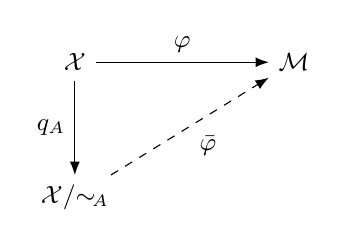
\begin{tikzpicture}[baseline=(current bounding box.center),
  node distance=1.8cm,
  every node/.style={font=\small}]
  \node (X) {$\calX$};
  \node (M) [right=2.2cm of X] {$\calM$};
  \node (Q) [below=1.2cm of X] {$\calX/{\simA}$};
  \draw[-Latex] (X) -- node[above]{$\varphi$} (M);
  \draw[-Latex] (X) -- node[left]{$q_A$} (Q);
  \draw[-Latex,dashed] (Q) -- node[below right]{$\bar{\varphi}$} (M);
\end{tikzpicture}
\end{equation}
where $\simA^*$ is the quotient relation on $\Xmod{A}$ induced by $\simA$.
Consequently, $q_A$ is the \emph{initial object} in the category of admissible
projections from $\calX$: every planning-safe representation factors uniquely
through the admissibility quotient.
\end{theorem}

\begin{proof}
\emph{Existence.} Define $\bar{\varphi}:[x]\mapsto\varphi(x)$ for each
equivalence class $[x]\in\Xmod{A}$. Since $\varphi$ is admissible, if
$x_1\simA x_2$ then $\varphi(x_1)=\varphi(x_2)$ (by
Definition~\ref{def:admissibility}), so $\bar{\varphi}$ is well-defined on
equivalence classes. By construction, $\bar{\varphi}(q_A(x))=\bar{\varphi}([x])=\varphi(x)$,
so $\varphi=\bar{\varphi}\circ q_A$.

\emph{Uniqueness.} Any $\psi:\Xmod{A}\to\calM$ satisfying $\varphi=\psi\circ q_A$
must satisfy $\psi([x])=\psi(q_A(x))=\varphi(x)$ for all $x$. Since every
element of $\Xmod{A}$ is of the form $[x]$, $\psi$ is uniquely determined.

\emph{Initiality.} A morphism $q_A:(\calX,\simA)\to(\Xmod{A},\simA^*)$ exists
and is universal: every morphism out of $(\calX,\simA)$ factors uniquely through
it. This is the defining property of an initial object in the slice category
over $\calM$.
\end{proof}

Theorem~\ref{thm:universal_prop} gives the admissibility quotient a character
stronger than "largest safe equivalence relation": it is the \emph{initial}
planning-safe abstraction, the one through which every other safe abstraction
necessarily factors. The factorisation map $\bar{\varphi}$ is unique, making the
relationship between any admissible representation and the admissibility quotient
canonical rather than constructed.

The categorical language also reframes admissibility distortion. $\DA$ measures
how far $\varphi$ is from being a morphism in $\mathbf{Adm}$: specifically, it
measures the expected reachability separation between pairs that $\varphi$
collapses but $\simA$ does not. A zero-distortion projection is a morphism; a
positive-distortion projection is a broken morphism whose degree of failure is
quantified by $\DA$.

The lattice structure of $\mathbf{Adm}$ connects to the Knuth--Skilling
programme \citep{knuth2012foundations}, which derives the sum and product rules
of probability as the unique consistent valuation on a distributive lattice
ordered by logical implication. The admissibility quotient lattice
$(\mathcal{X}/{\simA}, \subseteq)$, ordered by set inclusion of reachability
sets, is a distributive lattice of exactly this type. A valuation on this
lattice that assigns $0$ to admissibility-equivalent pairs and positive values
to inadmissible collapses is precisely $\DA$. The Knuth--Skilling uniqueness
result suggests that $\DA$, up to choice of severity metric $d$, is the
canonical measure of departure from morphism-hood in $\mathbf{Adm}$---the
unique consistent quantification of admissibility violation, just as probability
is the unique consistent quantification of logical implication on a distributive
lattice of propositions.

% ─────────────────────────────────────────────────────────────────────────
\section{Sheaf-Theoretic Reading of the Separation Theorem}
\label{app:sheaf}

We show that the Observational--Interventional Separation Theorem
(Theorem~\ref{thm:oi}) has a natural sheaf-theoretic interpretation: observation
provides sections of one sheaf while planning requires sections of a different
sheaf on a finer topology. The impossibility of recovering planning-relevant
information from observational data corresponds to a sheaf cohomological
obstruction.

\subsection*{Reachability Topology and the Planning Sheaf}

Define the \emph{reachability topology} $\tau_A$ on $\calX$ as the topology
generated by the reachability balls
\[
  B_H^\Pi(x) = \RHP(x) = \{y\in\calX : \exists\,\pi\in\Pi,\;
  x\overset{\pi,H}{\rightsquigarrow}y\},
\]
taking these as basic open sets. The topology $\tau_A$ captures which states
are "near" $x$ in the sense of being reachable from it.

Define the \emph{planning presheaf} $\mathcal{F}_A$ by assigning to each open
$U\in\tau_A$ the set of reachable futures from $U$:
\[
  \mathcal{F}_A(U) = \bigcup_{x\in U}\RHP(x),
\]
with restriction maps $\rho_{UV}:\mathcal{F}_A(U)\to\mathcal{F}_A(V)$ given by
inclusion for $V\subseteq U$.

\subsection*{Observation Topology and the Observation Sheaf}

Define the \emph{observation topology} $\tau_O$ on $\calX$ as generated by
observational indistinguishability neighborhoods:
\begin{multline*}
  N_O(x) = \bigl\{y\in\calX :
  P(O_{t+1:t+k}\mid y) = P(O_{t+1:t+k}\mid x)\\
  \text{for all } k\geq 1\bigr\}.
\end{multline*}
The observation sheaf $\mathcal{F}_O$ assigns to $U\in\tau_O$ the observation
distributions accessible from $U$:
\[
  \mathcal{F}_O(U) = \bigl\{P(O_{t+1:t+k}\mid x) :
  x\in U,\; k\geq 1\bigr\}.
\]

\subsection*{The Separation Theorem as a Sheaf Statement}

\begin{theorem}[Sheaf Formulation of Separation]
\label{thm:sheaf_sep}
The topologies $\tau_O$ and $\tau_A$ are distinct in general, with $\tau_O$ coarser
than $\tau_A$: observationally indistinguishable states may be reachability-distinguishable.
Consequently, a global section of $\mathcal{F}_A$ (complete reachability
information for all of $\calX$) is not determined by the sections of $\mathcal{F}_O$
(observational information on a $\tau_O$-cover). There exist covers $\{U_i\}$
of $\calX$ in $\tau_O$ on which local sections of $\mathcal{F}_O$ are compatible,
yet do not assemble into a section of $\mathcal{F}_A$.
\end{theorem}

\begin{proof}
By Theorem~\ref{thm:oi}, there exist $x_1,x_2\in\calX$ with $x_1\simO x_2$
(so $x_1$ and $x_2$ belong to the same $\tau_O$-neighborhood) but
$\RHP(x_1)\neq\RHP(x_2)$ (so $x_1$ and $x_2$ belong to different
$\tau_A$-basic-open-sets). Any $\tau_O$-cover of $\calX$ groups $x_1$ and $x_2$
into the same open set and assigns them the same local section of
$\mathcal{F}_O$. A global section of $\mathcal{F}_A$ must distinguish $x_1$
and $x_2$ (since their reachability sets differ), but no $\tau_O$-local
information can force this distinction. The attempted assembly of local
$\mathcal{F}_O$-sections into a global $\mathcal{F}_A$-section therefore
fails the uniqueness condition of the sheaf axiom: two distinct global
admissibility sections are consistent with the same observational local data.
\end{proof}

\begin{remark}[Interpretation]
Local sections of $\mathcal{F}_O$ correspond to passive observational data
available to a predictive learner. A global section of $\mathcal{F}_A$
corresponds to complete knowledge of the reachability geometry required for
planning. Theorem~\ref{thm:sheaf_sep} establishes that observation provides
local sections of $\mathcal{F}_O$, while planning requires a global section of
$\mathcal{F}_A$, and these are sections of different sheaves on different
topologies. The failure of local-to-global assembly is precisely the
observational--interventional gap: locally consistent observation does not
determine globally consistent reachability.
\end{remark}

The failure of assembly can be understood as a cohomological obstruction: the
mismatch between $\tau_O$ and $\tau_A$ produces a non-trivial \v{C}ech
cohomology class $[\delta s]\in H^1(\tau_O;\mathcal{F}_A)$ that obstructs
extension of local $\mathcal{F}_O$-sections to global $\mathcal{F}_A$-sections.
Formalising this obstruction class and connecting it to the mutual-information
bound $I(A;\varphi(X))$ of Theorem~\ref{thm:guardrail} is a natural direction
for future work: the magnitude of the obstruction may be quantifiable in terms
of $\DA$.

\subsection*{Temporal Admissibility as a Sheaf over Time}

The dynamic state-space setting of Appendix~\ref{app:dynamic} also admits a
sheaf-theoretic reading. Let the base category be the poset of time intervals
$[s,t]$ ordered by inclusion. Assign to each interval $[s,t]$ the admissibility
structure $(\calX_{[s,t]},\sim_A^{[s,t]})$ on the time-slice of state space. The
restriction maps are the transition functions $F:\calX_t\to\calX_{t+1}$ of
Appendix~\ref{app:dynamic}. Meta-admissibility (Definition in
Appendix~\ref{app:dynamic}) is then precisely the sheaf compatibility condition:
sections on overlapping time intervals agree on their overlap. The composition
theorem (Proposition~\ref{prop:compose}) is the sheaf gluing lemma for this
temporal sheaf: compatible local admissibility structures assemble into a global
admissibility structure over the developmental trajectory. A developmental
transition that violates meta-admissibility corresponds to a failed gluing,
creating a cohomological obstruction to consistent identity over time.

% ═══════════════════════════════════════════════════════════════════════════
% BIBLIOGRAPHY
% ═══════════════════════════════════════════════════════════════════════════

\begin{thebibliography}{99}

\bibitem[Bertsekas(2012)]{bertsekas2012dynamic}
Bertsekas, D.~P. (2012).
\textit{Dynamic Programming and Optimal Control}, Vol.~1, 4th ed.
Athena Scientific.

\bibitem[Blum \& Blum(2022)]{blum2022conscious}
Blum, L., \& Blum, M. (2022).
A theoretical computer science perspective on consciousness.
\textit{Journal of Artificial Intelligence and Consciousness}, 9(1), 1--42.

\bibitem[Castro \& Precup(2010)]{castro2010bisimulation}
Castro, P.~S., \& Precup, D. (2010).
Using bisimulation for policy transfer in MDPs.
\textit{AAAI}.

\bibitem[Cover \& Thomas(2006)]{cover2006elements}
Cover, T.~M., \& Thomas, J.~A. (2006).
\textit{Elements of Information Theory}, 2nd ed.
Wiley.

\bibitem[Craik(1943)]{craik1943nature}
Craik, K.~J.~W. (1943).
\textit{The Nature of Explanation}.
Cambridge University Press.

\bibitem[Dayan(1993)]{dayan1993improving}
Dayan, P. (1993).
Improving generalisation for temporal difference learning: The successor
representation.
\textit{Neural Computation}, 5(4), 613--624.

\bibitem[Ferns et al.(2004)]{ferns2004metrics}
Ferns, N., Panangaden, P., \& Precup, D. (2004).
Metrics for finite Markov decision processes.
\textit{UAI}, 162--169.

\bibitem[Fisher(1922)]{fisher1922mathematical}
Fisher, R.~A. (1922).
On the mathematical foundations of theoretical statistics.
\textit{Phil.\ Trans.\ Roy.\ Soc.\ A}, 222, 309--368.

\bibitem[Garcia et al.(1989)]{garcia1989model}
Garcia, C.~E., Prett, D.~M., \& Morari, M. (1989).
Model predictive control: Theory and practice.
\textit{Automatica}, 25(3), 335--348.

\bibitem[Gibson(1979)]{gibson1979ecological}
Gibson, J.~J. (1979).
\textit{The Ecological Approach to Visual Perception}.
Houghton Mifflin.

\bibitem[Graziano(2013)]{graziano2013consciousness}
Graziano, M.~S.~A. (2013).
\textit{Consciousness and the Social Brain}.
Oxford University Press.

\bibitem[Rao et al.(2026)]{rao2026decoupled}
Rao, M.~P., Pacheco-Solana, A., Li, R., et al. (2026).
Decoupled carbon assimilation and growth responses to aridity in temperate
deciduous oaks.
\textit{Science Advances}, 12, eady7139.

\bibitem[Gupta \& Pruthi(2025)]{gupta2025world}
Gupta, T., \& Pruthi, D. (2025).
Beyond world models: Rethinking understanding in AI models.
\textit{arXiv}:2511.12239.

\bibitem[Jaynes(2003)]{jaynes2003probability}
Jaynes, E.~T. (2003).
\textit{Probability Theory: The Logic of Science}.
Cambridge University Press.

\bibitem[Knuth \& Skilling(2012)]{knuth2012foundations}
Knuth, K.~H., \& Skilling, J. (2012).
Foundations of inference.
\textit{Axioms}, 1(1), 38--73.

\bibitem[Kaelbling et al.(1998)]{kaelbling1998planning}
Kaelbling, L.~P., Littman, M.~L., \& Cassandra, A.~R. (1998).
Planning and acting in partially observable stochastic domains.
\textit{Artificial Intelligence}, 101(1--2), 99--134.

\bibitem[Kalman(1960)]{kalman1960general}
Kalman, R.~E. (1960).
On the general theory of control systems.
\textit{Proc.\ First IFAC Congress}, 481--492.

\bibitem[Kemertas \& Aumentado-Armstrong(2021)]{kemertas2021towards}
Kemertas, M., \& Aumentado-Armstrong, T. (2021).
Towards robust bisimulation metric learning.
\textit{NeurIPS}, 34.

\bibitem[Li et al.(2006)]{li2006towards}
Li, L., Walsh, T.~J., \& Littman, M.~L. (2006).
Towards a unified theory of state abstraction for MDPs.
\textit{ISAIM}, 531--539.

\bibitem[Littman et al.(2002)]{littman2002predictive}
Littman, M.~L., Sutton, R.~S., \& Singh, S. (2002).
Predictive representations of state.
\textit{NeurIPS}, 14.

\bibitem[Ljung(1999)]{ljung1999system}
Ljung, L. (1999).
\textit{System Identification: Theory for the User}, 2nd ed.
Prentice Hall.

\bibitem[Mayne et al.(2000)]{mayne2000model}
Mayne, D.~Q., Rawlings, J.~B., Rao, C.~V., \& Scokaert, P.~O.~M. (2000).
Constrained model predictive control: Stability and optimality.
\textit{Automatica}, 36(6), 789--814.

\bibitem[van den Oord et al.(2018)]{oord2018representation}
van den Oord, A., Li, Y., \& Vinyals, O. (2018).
Representation learning with contrastive predictive coding.
\textit{arXiv}:1807.03748.

\bibitem[Pearl(2009)]{pearl2009causality}
Pearl, J. (2009).
\textit{Causality: Models, Reasoning, and Inference}, 2nd ed.
Cambridge Univ.\ Press.

\bibitem[Poincar\'e(1914)]{poincare1914}
Poincar\'e, H. (1914).
\textit{Science and Method}.
Thomas Nelson.

\bibitem[Popper(1979)]{popper1979objective}
Popper, K.~R. (1979).
\textit{Objective Knowledge}.
Clarendon Press.

\bibitem[Ravindran \& Barto(2004)]{ravindran2004algebraic}
Ravindran, B., \& Barto, A.~G. (2004).
Approximate homomorphisms: A framework for non-exact minimization in MDPs.
\textit{KBCS}.

\bibitem[Schmidhuber(1991)]{schmidhuber1991possibility}
Schmidhuber, J. (1991).
A possibility for implementing curiosity and boredom.
\textit{SAB}, 222--227.

\bibitem[Schmidhuber(2010)]{schmidhuber2010formal}
Schmidhuber, J. (2010).
Formal theory of creativity, fun, and intrinsic motivation.
\textit{IEEE Trans.\ Auton.\ Mental Dev.}, 2(3), 230--247.

\bibitem[Sutton et al.(2011)]{sutton2011horde}
Sutton, R.~S., et al. (2011).
Horde: A scalable real-time architecture for learning knowledge.
\textit{AAMAS}, 761--768.

\bibitem[Tishby et al.(1999)]{tishby1999information}
Tishby, N., Pereira, F.~C., \& Bialek, W. (1999).
The information bottleneck method.
\textit{Allerton}, 368--377.

\bibitem[Tomlin et al.(2003)]{tomlin2003computational}
Tomlin, C.~J., Mitchell, I., Bayen, A.~M., \& Oishi, M. (2003).
Computational techniques for verification of hybrid systems.
\textit{Proc.\ IEEE}, 91(7), 986--1001.

\bibitem[Varela et al.(1999)]{varela1999first}
Varela, F.~J., Shear, J., \emph{et al.} (Eds.) (1999).
\textit{The View from Within: First-Person Approaches to the Study of Consciousness}.
Imprint Academic.

\bibitem[V\'eliz(2024)]{veliz2024prophecy}
V\'eliz, C. (2024).
\textit{Prophecy: The Power and Perils of Looking into the Future}.
Oxford Univ.\ Press.

\bibitem[Wilson(1975)]{wilson1975renormalization}
Wilson, K.~G. (1975).
The renormalization group: Critical phenomena and the Kondo problem.
\textit{Rev.\ Mod.\ Phys.}, 47(4), 773--840.

\bibitem[Zhang et al.(2021)]{zhang2021learning}
Zhang, A., McAllister, R., Calandra, R., Gal, Y., \& Levine, S. (2021).
Learning invariant representations for RL without reconstruction.
\textit{ICLR}.

\end{thebibliography}

\end{document}
